\section{Extruding PLCL\label{methodology:extrudingPLCL}}

\subsection{Summary of PLCL Extrusions\label{methodology:extrudingPLCL:plclSummary}}

A significant portion of the research in this thesis pertains to extruding PLCL into a 3D printable filament. Multiple methods were employed to eventually achieve this. In summary, powder extrusions were first attempted. This was followed by manually and then automatically combining PLA and PCL pellets in a single screw extruder. Two extruders, 3Devo Filament Maker 1 and the Felfil Evo, were used to conduct these extrusions. Finally, shredding or regrinding the initial PLCL output and re-extruding was tested to address thickness tolerance concerns. Figure~\ref{methodology:extrudingPLCL:plclSummary} outlines this process at a high level.

\begin{figure}[h!]
        \centering
        \includegraphics[width=\linewidth]{../figs/methodology/plclExtrusions/plcl_extrusion_summary.png}
        \caption{Overview of the progression of PLCL extruding research.}
        \label{fig:methodology:extrudingPLCL:plclSummary}
\end{figure}

Additionally,~\fullref{tab:appendix:extrusionSummary} details all extrusions performed and their results.

\subsection{Powder Extrusions\label{sec:methodology:extrudingPLCL:powderExtrusion}}

Based on material availability, the team attempted to extrude PLCL powder to create PLCL filament. While pellets are more commonly extruded than powders(See~\fullref{sec:literatureReview:extrusion:powder}), the team was unable to source PLCL pellets at a scalable price. As a result, Nomisma PLCL powder was used~\cite{RefWorks:RefID:387-nomisma} for these initial extrusions on a 3Devo Filament Maker 1 single screw extruder.

Prior to extruding, the PLCL powder was dried in a vaccuum oven at 45\textcelsius ~overnight based on the material manufacturer's recommendations. The Polymer Synthesis Research Facility (PSRF) at Ohio State University was utilized for this task (see~\fullref{sec:methodology:externalLabs:polymersLab} for more information on research conducted with this additional lab).

The powder was measured and poured into the extruder as shown in Figure~\ref{fig:methodology:extrudingPLCL:powderExtrusion}.

\begin{figure}[h!]
        \centering
        \includegraphics[width=0.7\linewidth]{../figs/methodology/plclExtrusions/powderExtrusion/powder_extrusion.png}
        \caption{Performing PLCL powder extrusion. Measuring powder (left) and pouring into extruder (right).}
        \label{fig:methodology:extrudingPLCL:powderExtrusion}
\end{figure}

In addition to pouring the powder, a pusher inspired by the Devostick was employed~\cite{RefWorks:RefID:396-3devotroubleshooting}. This is a rectangular piece of wood used to compress the material in hopes of resolving feeding issues. Using the pusher piece is shown below in ~\autoref{fig:methodology:extrudingPLCL:devostick}.

\begin{figure}[h!]
        \centering
        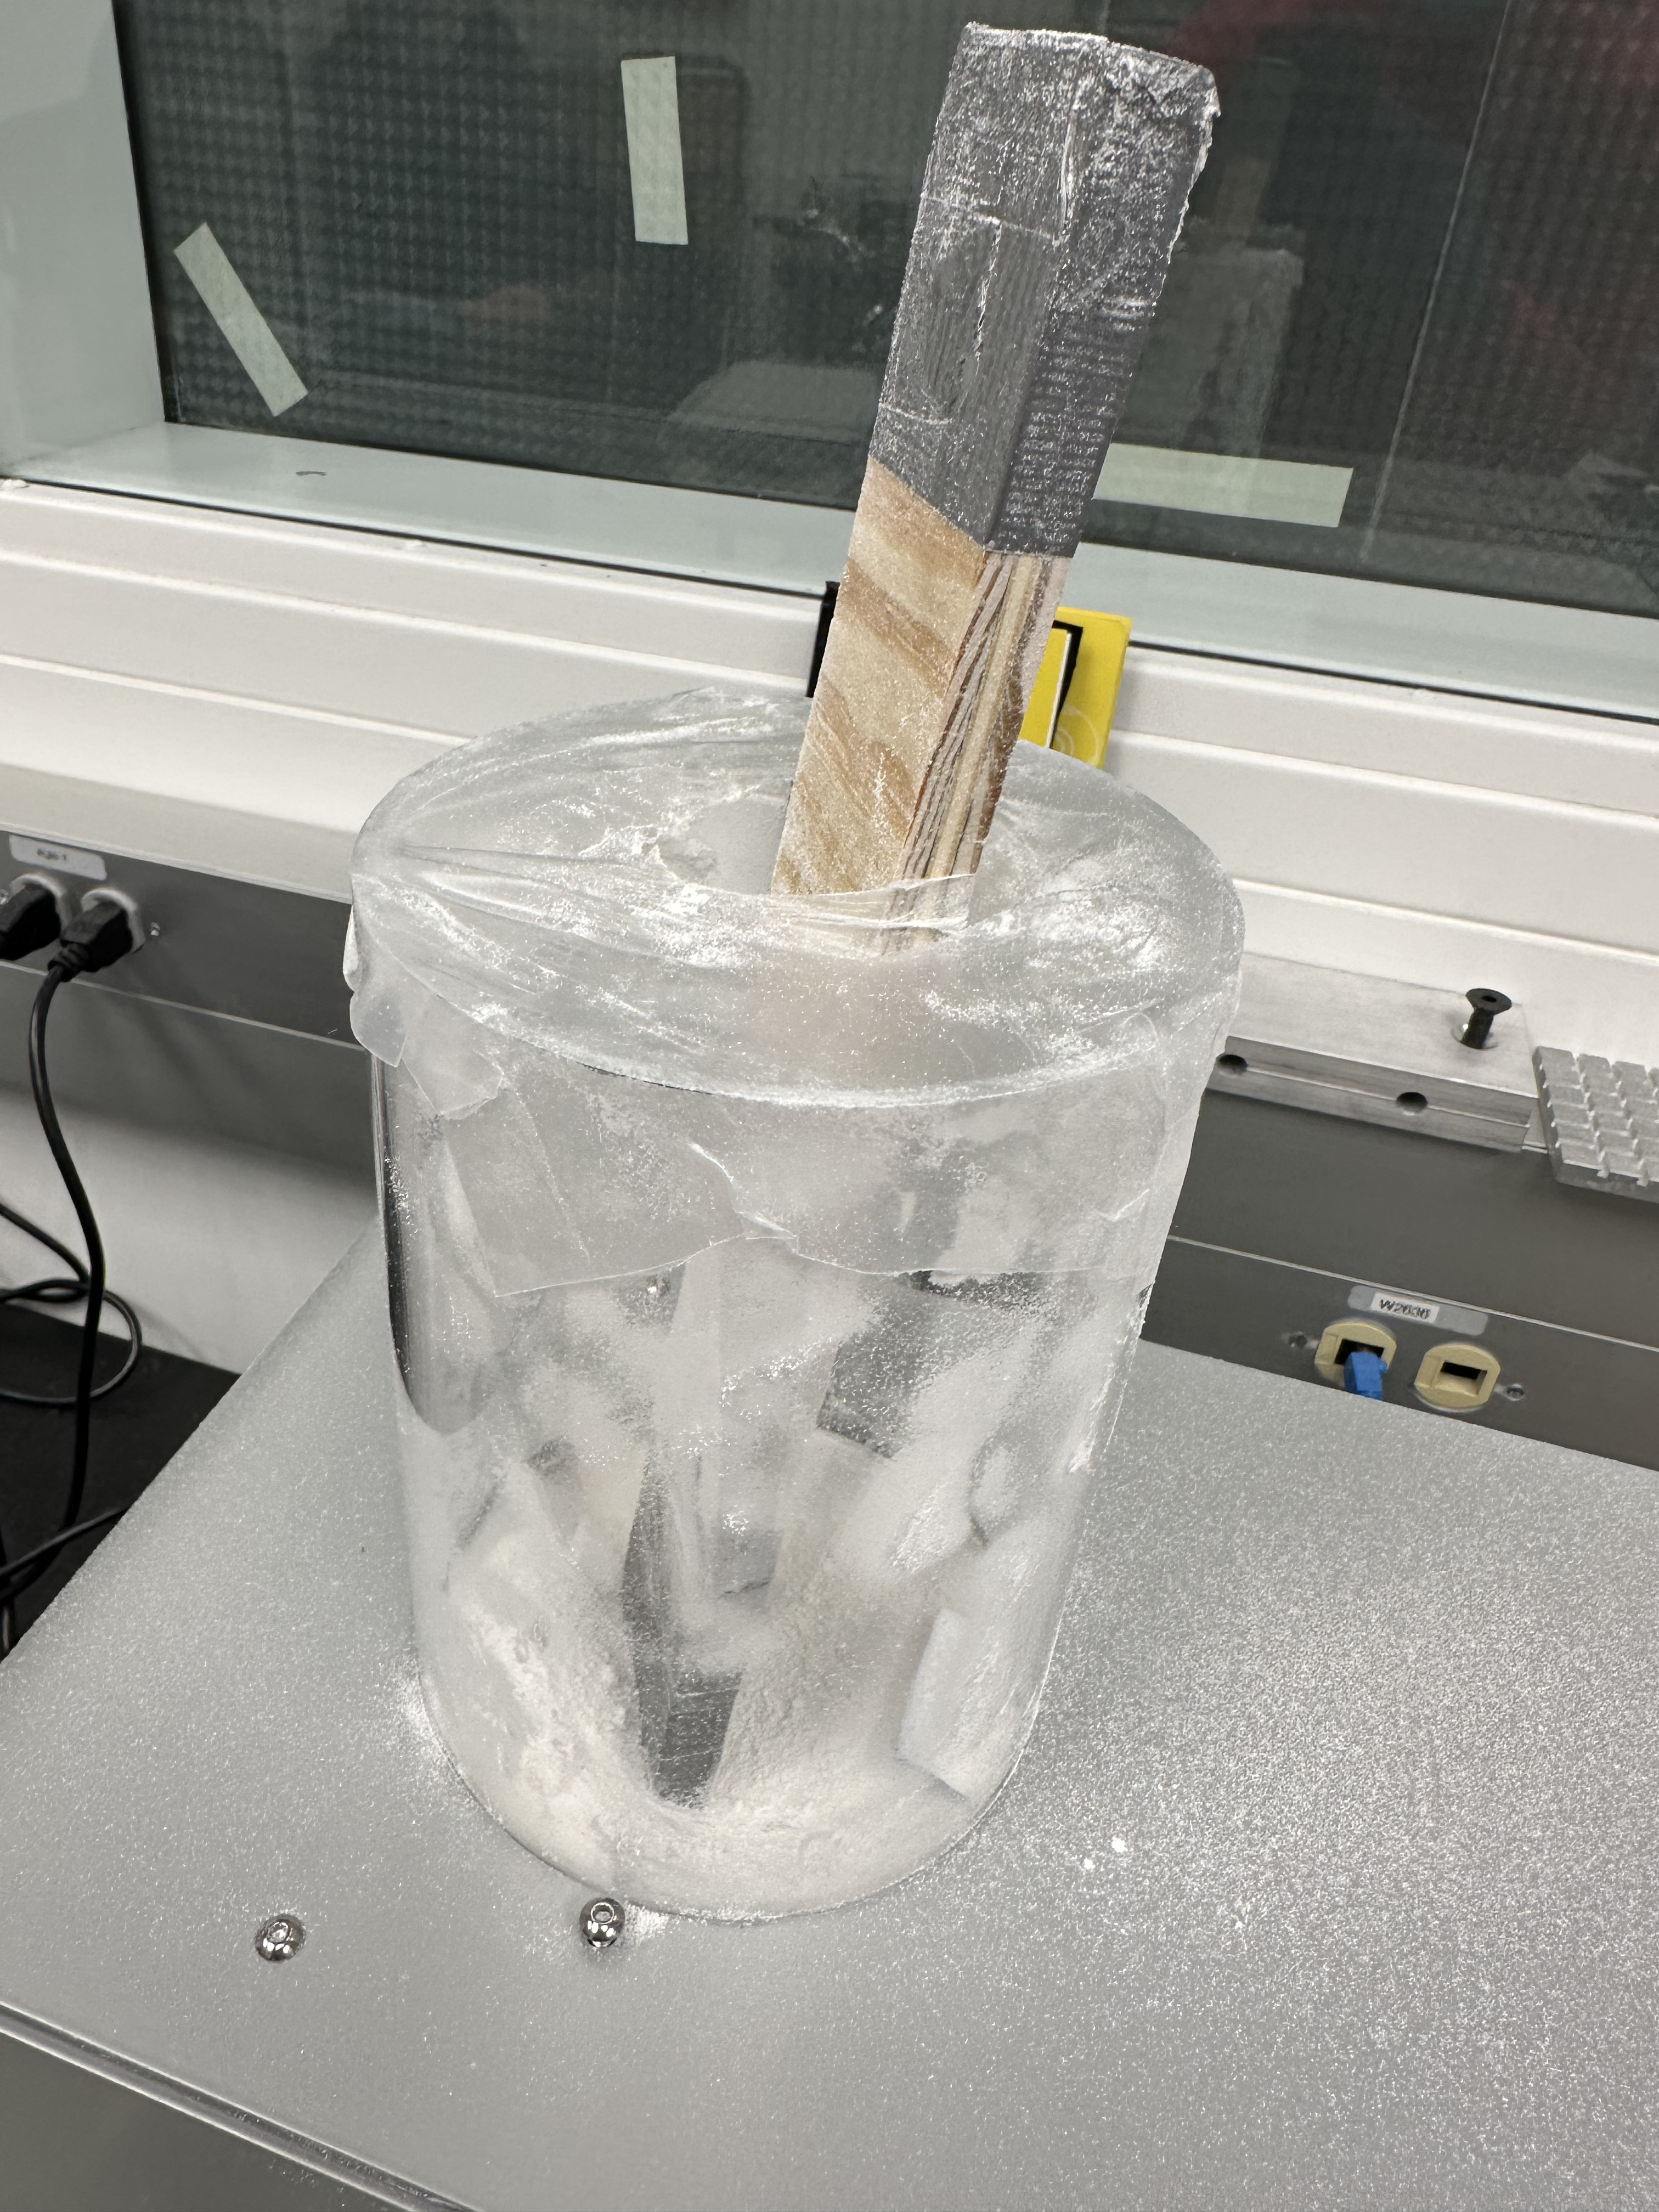
\includegraphics[width=0.5\linewidth]{../figs/methodology/plclExtrusions/powderExtrusion/devostick.png}
        \caption{Using the self-made "Devostick".}
        \label{fig:methodology:extrudingPLCL:devostick}
\end{figure}

This extruder has four heat zones with heater 4 (H4) being closest to the hopper and heater 1 (H1) being closest to the nozzle. Heaters 4 through 1 were set to 205\textcelsius, 200\textcelsius, 195\textcelsius, and 190\textcelsius ~respectively based on 3Devo customer support recommendations. The RPM for the extruder was set to 3.5.

To achieve these temperatures, the extruder was first run at PLA presets (H4-H1: 170, 185, 190, 170 (all in \textcelsius)). Temperatures were raised to HDPE presets (190\textcelsius ~across all heat zones) and HDPE was introduced into the extruder. Finally, temperatures were raised to the PLCL extruding temperatures and the PLCL powder was introduced into the extruder. DevoVision was used to monitor extruder parameters and variables such as current and heater temperatures.

The results and discussion for this experiment can be found in~\fullref{results:extrudingPLCL:powderExtrusion} and~\fullref{discussion:extrudingPLCL:powderExtrusion} respectively.

\subsection{Combining Raw Materials\label{sec:methodology:extrudingPLCL:combiningMaterials}}

\subsubsection{College of Pharmacy\label{sec:methodology:extrudingPLCL:combiningMaterials:pharmacy}}

\subsubsection{Injection Molding\label{sec:methodology:extrudingPLCL:combiningMaterials:injectionMolding}}

\subsubsection{Chemically Combining Materials\label{sec:methodology:extrudingPLCL:combiningMaterials:chemicallyCombining}}
% Requires toxic chemicals (MDF or chloroform)
% Tried melting materials together using hotplate
% Difficult to get shape that is easily shred able

\subsubsection{3D Printable Mixing Systems\label{sec:methodology:extrudingPLCL:combiningMaterials:3dPrintedMixers}}

\subsubsection{Discussion with ISE Department\label{sec:methodology:extrudingPLCL:combiningMaterials:iseDiscussion}}
% Met with Dr. Mulyana at ISE
% We can just combine in a bag

% iii.	Purging Compounds
% 1.	Found initial supplier of 3Devo DevoClean Mid-Temp
% 2.	Worked with supplier (Dyna-Purge) to find ideal purging material
% a.	Tried L then D2 (needs HDPE) then K

\subsection{Purging Compounds\label{sec:methodology:extrudingPLCL:purgingCompounds}}

\subsubsection{Initial Purging Process\label{sec:methodology:extrudingPLCL:purgingCompounds:initialProcess}}

\subsubsection{Supplier Discovery\label{sec:methodology:extrudingPLCL:purgingCompounds:supplierDiscovery}}

\subsubsection{Dyna-Purge Collaboration\label{sec:methodology:extrudingPLCL:purgingCompounds:dynaPurgeCollaboration}}
% Tried L then D2 (needs HDPE) then K

\hl{[Add more about successful PLCL extrusions, too thin on 3Devo so I went to Felfil now that we're using pellets instead of powders.]}

\subsection{Felfil System\label{sec:methodology:extrudingPLCL:felfilSystem}}

\subsubsection{Felfil Evo Initial Testing\label{sec:methodology:extrudingPLCL:felfilSystem:felfilEvo}}

\paragraph*{Initial Repairs\label{sec:methodology:extrudingPLCL:felfilSystem:felfilEvo:initialRepairs}}
% a. Tried replacing the hopper without fully disassembling
% b. Led to the barrel not being secured and spinning out of place
% c. Disassembled fully, cleaned, and reassembled correctly
% d. Replaced broken O-ring in nozzle

\paragraph*{Initial PLA Testing\label{sec:methodology:extrudingPLCL:felfilSystem:felfilEvo:initialTesting}}
% a. Tested with PLA pellets which worked wonderfully

\paragraph*{Learnings from Initial Testing\label{sec:methodology:extrudingPLCL:felfilSystem:felfilEvo:learningsFromInitialTesting}}
% a. Pellets remain the best material to extrude with
% b. Even though we couldn't get the system to work with powders, it can likely work well with pellets

\subsubsection{Felfil Evo PLCL Extrusion\label{sec:methodology:extrudingPLCL:felfilSystem:felfilEvoPLCL}}

\paragraph*{Initial PLCL Extrusion Attempts\label{sec:methodology:extrudingPLCL:felfilSystem:felfilEvoPLCL:initialAttempts}}
% a. Can extrude PLCL at proper thickness on 1st pass and faster than 3Devo
% b. First time we've had successul proper thickness PLCL filament

\paragraph*{Clumping at Hopper\label{sec:methodology:extrudingPLCL:felfilSystem:felfilEvoPLCL:clumpingAtHopper}}
% a. Noticed clumping at hopper due to metal wall closest to barrel
% b. Tried using starve feeding method but would need refining/testing
% c. Planned to look into isolating that metal wall section from the raw materials

\subsubsection{Felfil Evo Hopper Improvements\label{sec:methodology:extrudingPLCL:felfilSystem:felfilEvoHopperImprovements}}

\paragraph*{Silicone Coating\label{sec:methodology:extrudingPLCL:felfilSystem:felfilEvoHopperImprovements:siliconeCoating}}
% a. Looked into silicone with adhesive backing to block the heat (like what's used in Rasbperry Pi)
% b. Talked with Chris in electronics lab to see if he's run across that ever
% c. Initial google search on available materials

\paragraph*{3D Printed Hopper Insert\label{sec:methodology:extrudingPLCL:felfilSystem:felfilEvoHopperImprovements:3dPrintedHopperInsert}}
% a. Created a 3D printed insert to block the heat transfer
% b. Modeled it in SolidWorks after using the existing CAD files to create an assembly of the hopper
% c. Took 5 versions to properly account for the screw (couldn't measure by hand without fully disassembling machine)
% d. Added thickness and slope to address thin insert still getting hot
% i. Add distance between wall and raw materials

\subsubsection{Felfil Spooler+\label{sec:methodology:extrudingPLCL:felfilSystem:felfilSpooler}}

\paragraph*{Noticed Need to Log Thickness\label{sec:methodology:extrudingPLCL:felfilSystem:felfilSpooler:noticedNeedToLogThickness}}
% a. Realized I needed to log thickness data to analyze it like DevoVision does

\paragraph*{Accessing Firmware\label{sec:methodology:extrudingPLCL:felfilSystem:felfilSpooler:accessingFirmware}}
% a. Felfil is open source and run on an Arduino Nano
% b. I was able to access the current firmware (V1.8) and modify it
% c. USB-MiniB port is accessible through side of spooler or by taking casing off

\paragraph*{Modifying Firmware\label{sec:methodology:extrudingPLCL:felfilSystem:felfilSpooler:modifyingFirmware}}
% a. I looked through the firmware and found where the live diameter reading was stored
% b. Started by printing to serial monitor
% c. Created python script to store readings in a csv for easy logging and graphical analysis

\subsubsection{Felfil Shredder\label{sec:methodology:extrudingPLCL:felfilSystem:felfilShredder}}
% a. Started by shredding multiple times until regrind size looked uniform
% b. Downloaded sieve from Felfil to control for size and make sure everything is ~5mm x 5mm
% c. Discovered that medium-thick filament shreds best

\subsection{PLA with Barium Sulfate\label{sec:methodology:extrudingPLCL:plaWithBaSO4}}
